\chapter{Appendix}
\section{Transfer Learning}
\graphicspath{{figs/2a/}}
\subsection{Activation maps} \label{appendix:activation_maps}

\begin{figure}[H]
    \centering
    \includegraphics*[width=0.95\textwidth]{activation_dog}
    \caption{Activation maps obtanied after the first convolutional layer, on the Shih Tzu dog image}
    \label{fig:activation_dog}
\end{figure} 

\begin{figure}[H]
    \centering
    \includegraphics*[width=0.95\textwidth]{activation_komondor}
    \caption{Activation maps obtanied after the first convolutional layer, on the Komondor dog image}
    \label{fig:activation_komondor}
\end{figure} 

\begin{figure}[H]
    \centering
    \includegraphics*[width=0.95\textwidth]{activation_komondor_or_mop}
    \caption{Activation maps obtanied after the first convolutional layer, on the "Komondor or mop?" image}
    \label{fig:activation_komondor_or_mop}
\end{figure} 

\begin{figure}[H]
    \centering
    \includegraphics*[width=0.95\textwidth]{activation_wombat}
    \caption{Activation maps obtanied after the first convolutional layer, on the wombat image}
    \label{fig:activation_wombat}
\end{figure} 

\begin{figure}[H]
    \centering
    \includegraphics*[width=0.95\textwidth]{activation_dog_meme}
    \caption{Activation maps obtanied after the first convolutional layer, on the dog (meme) image}
    \label{fig:activation_dog_meme}
\end{figure} 

\subsection{Going further: VisionTransformer} \label{appendix:vit}

\begin{figure}[H]
    \centering
    \begin{subfigure}{0.95\textwidth}
        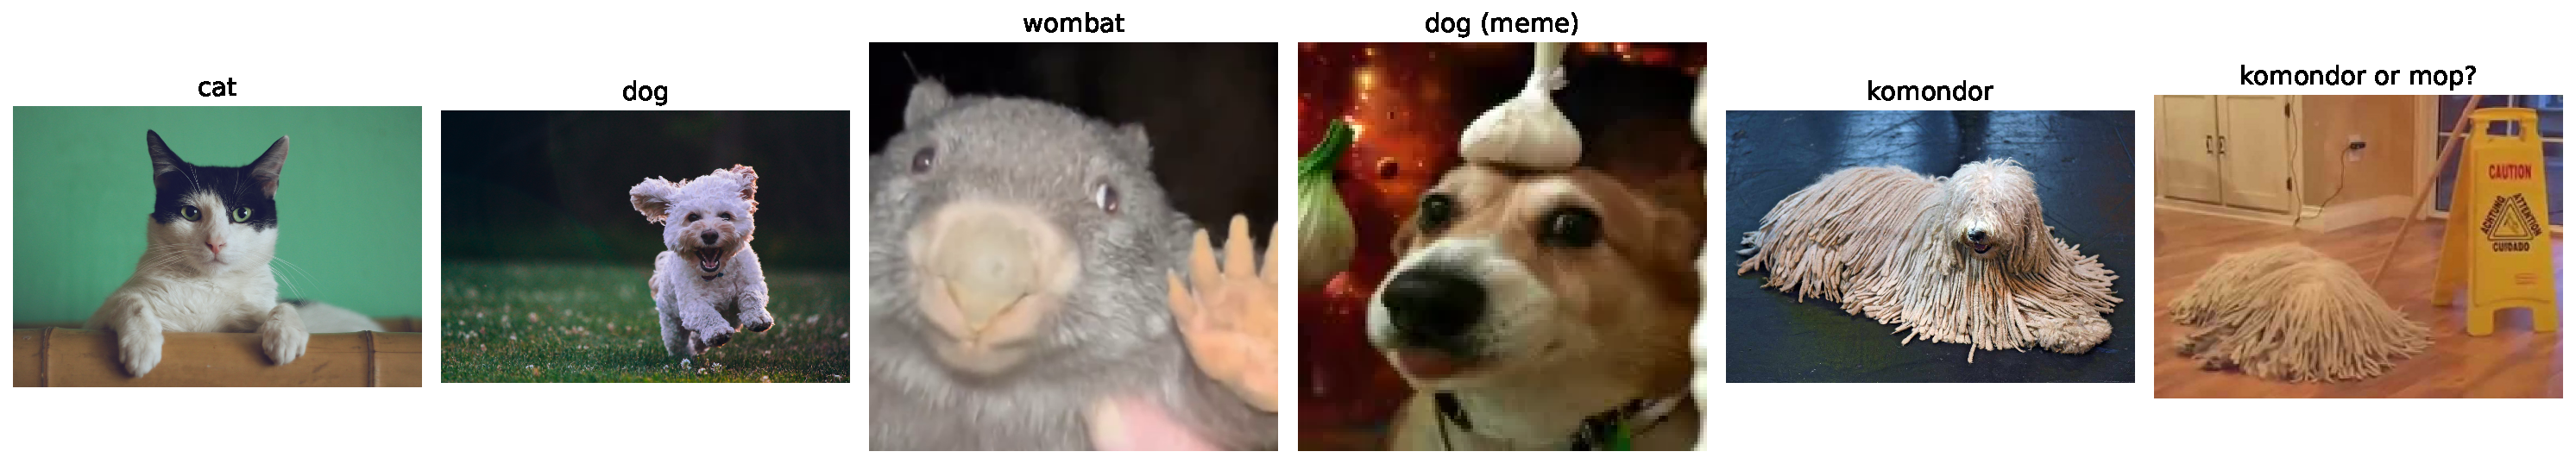
\includegraphics[width=\textwidth]{original_images_vit}
        \caption{}
        \label{subfig:original_images_vit}
    \end{subfigure}
    \begin{subfigure}{0.95\textwidth}
        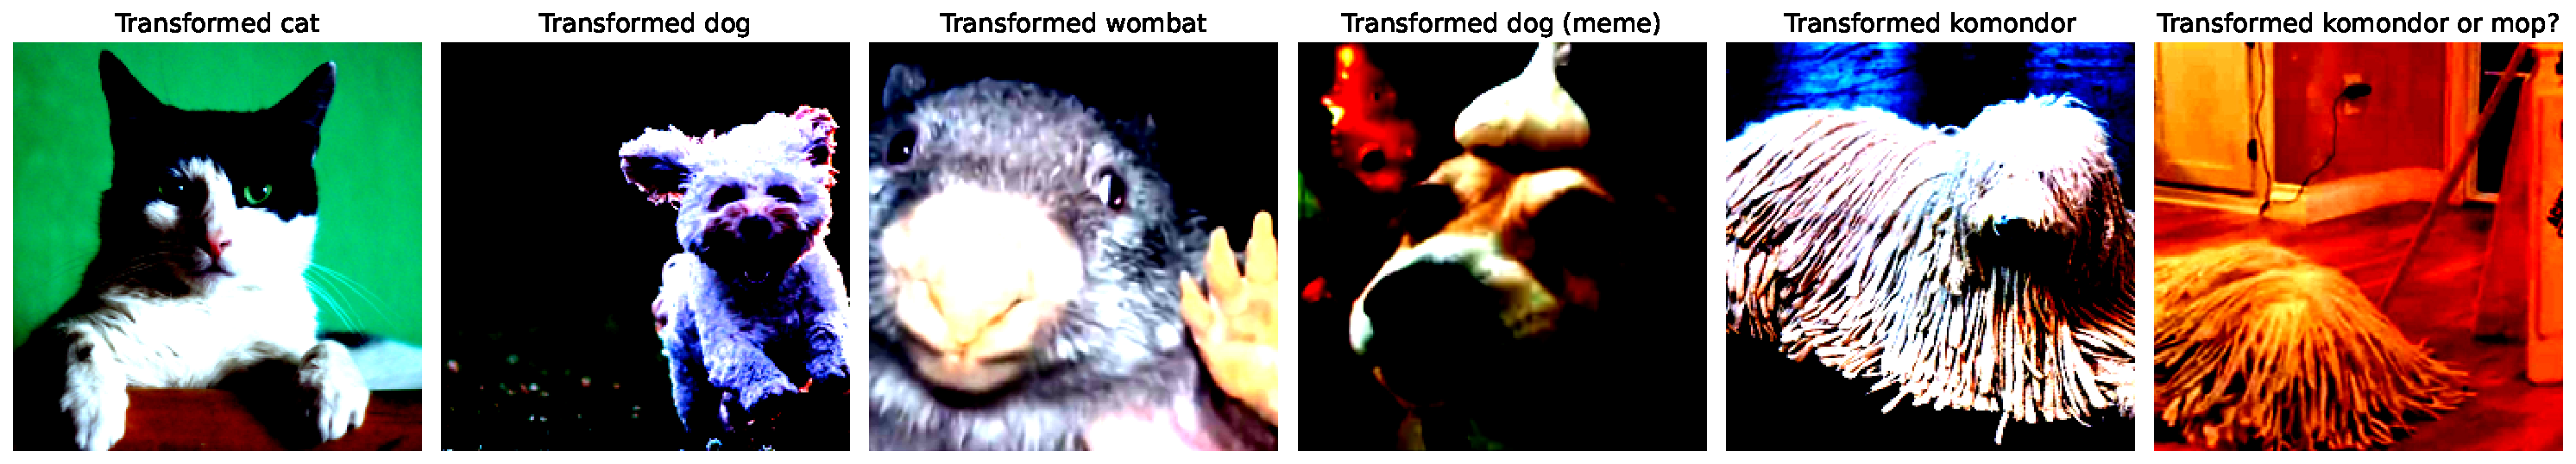
\includegraphics[width=\textwidth]{transformed_images_vit}
        \caption{}
        \label{subfig:transformed_images_vit}
    \end{subfigure}
    \begin{subfigure}{0.95\textwidth}
        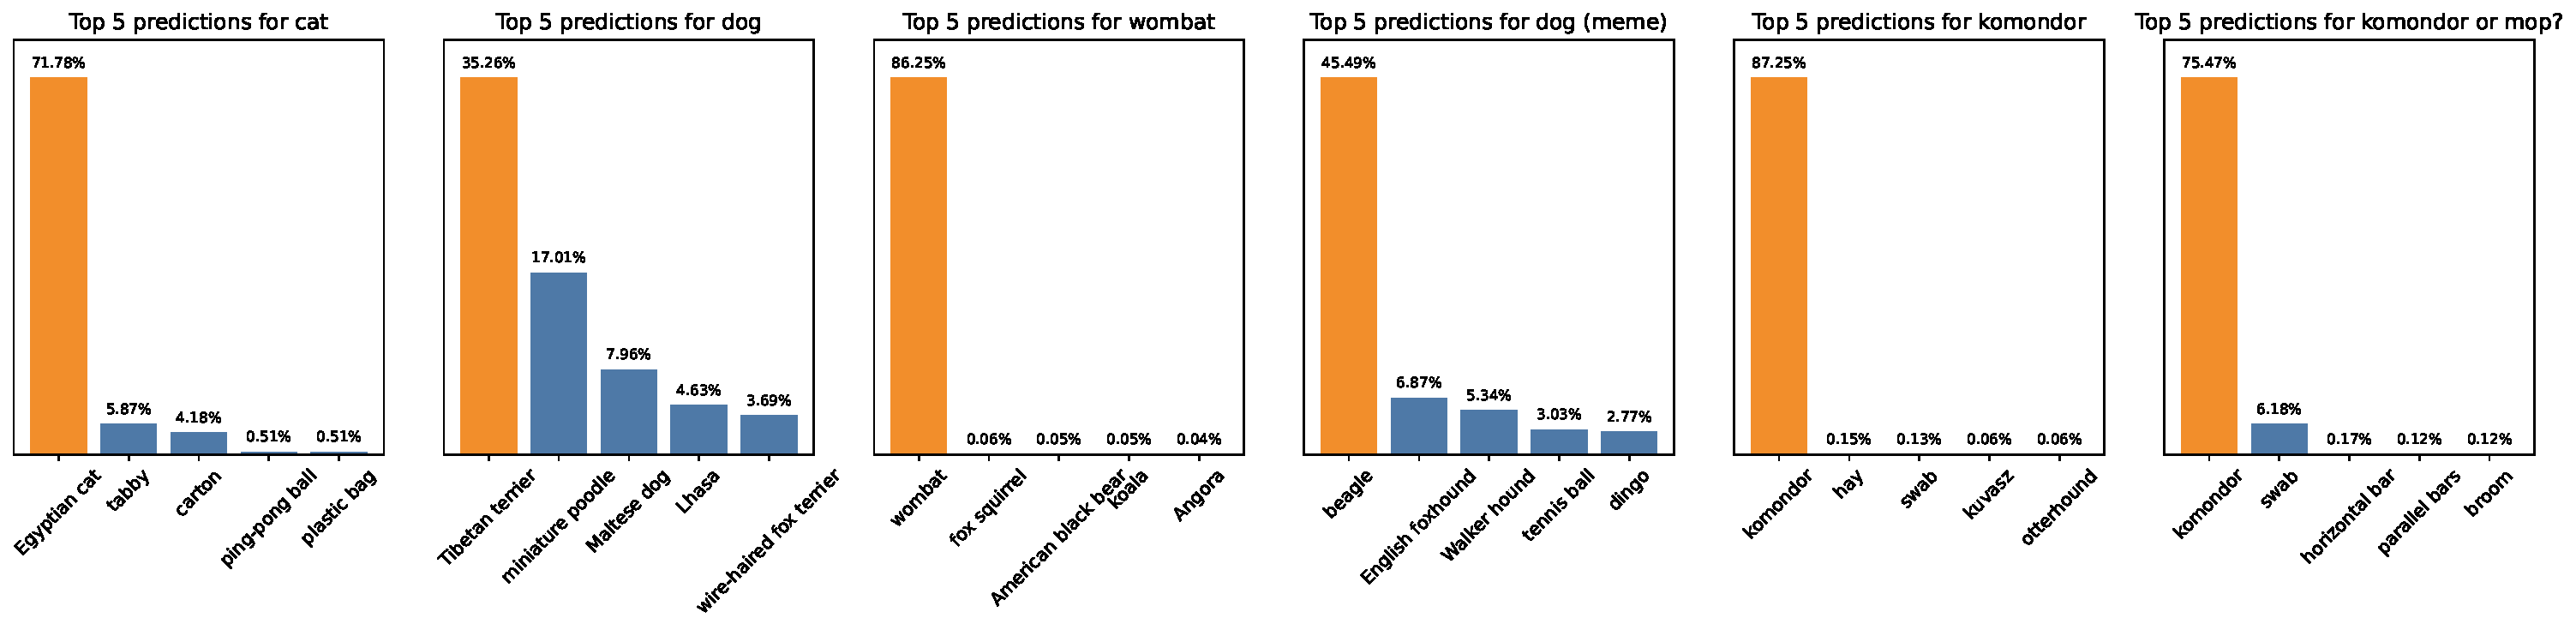
\includegraphics[width=\textwidth]{prediction_plots_vit}
        \caption{}
        \label{subfig:prediction_plots_vit}
    \end{subfigure}
    \caption{Performance evaluation of VisionTransformer pre-trained on ImageNet (IMAGENET1K\_V1 weights): (a) Original images, (b) Transformed images normalized and resized to $224 \times 224$, and (c) Top 5 predicted classes}
    \label{fig:vit_scratch}
\end{figure}

\begin{figure}[H]
    \centering
    \begin{subfigure}{0.95\textwidth}
        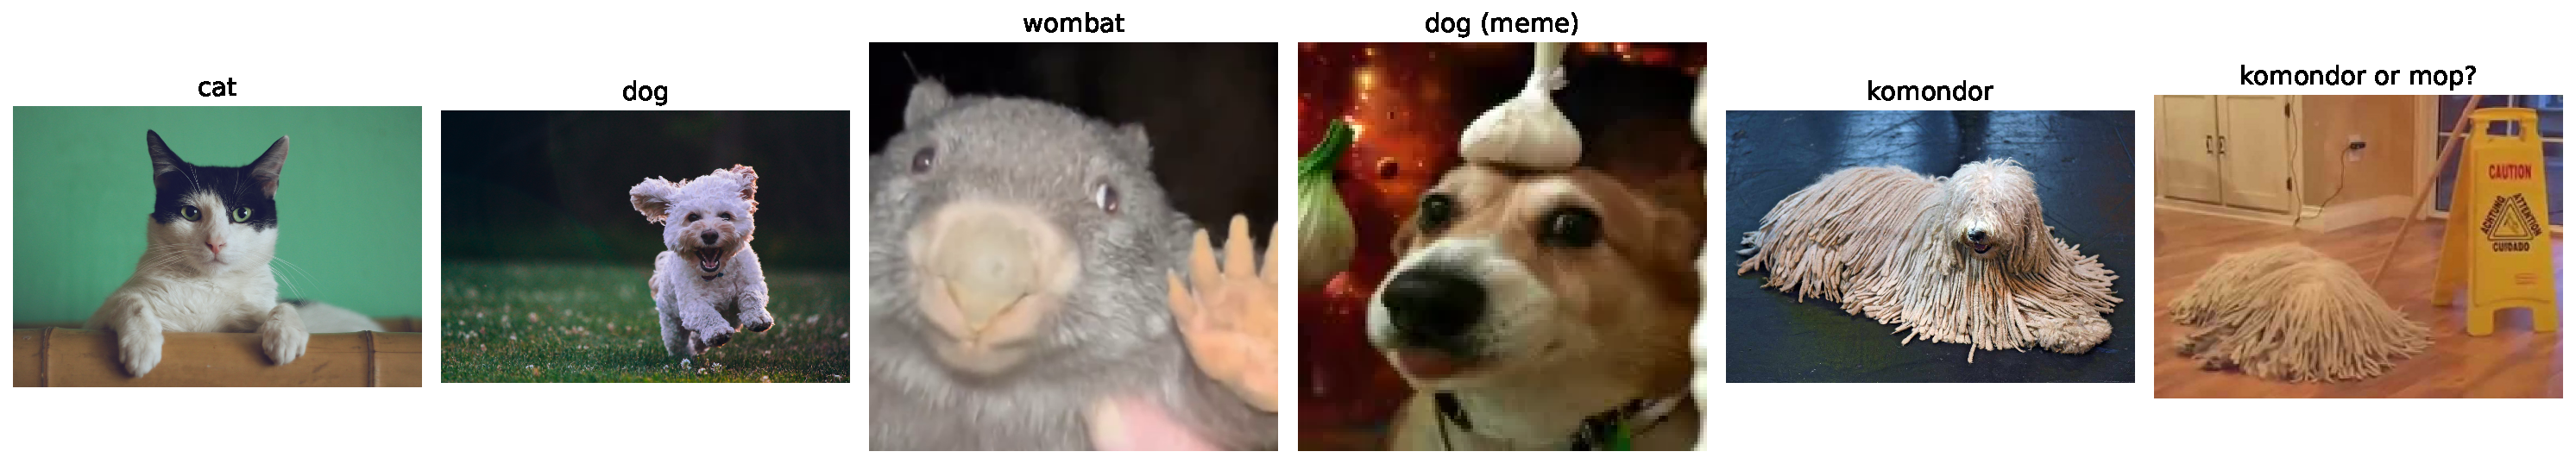
\includegraphics[width=\textwidth]{original_images_vit_bis}
        \caption{}
        \label{subfig:original_images_vit_bis}
    \end{subfigure}
    \begin{subfigure}{0.95\textwidth}
        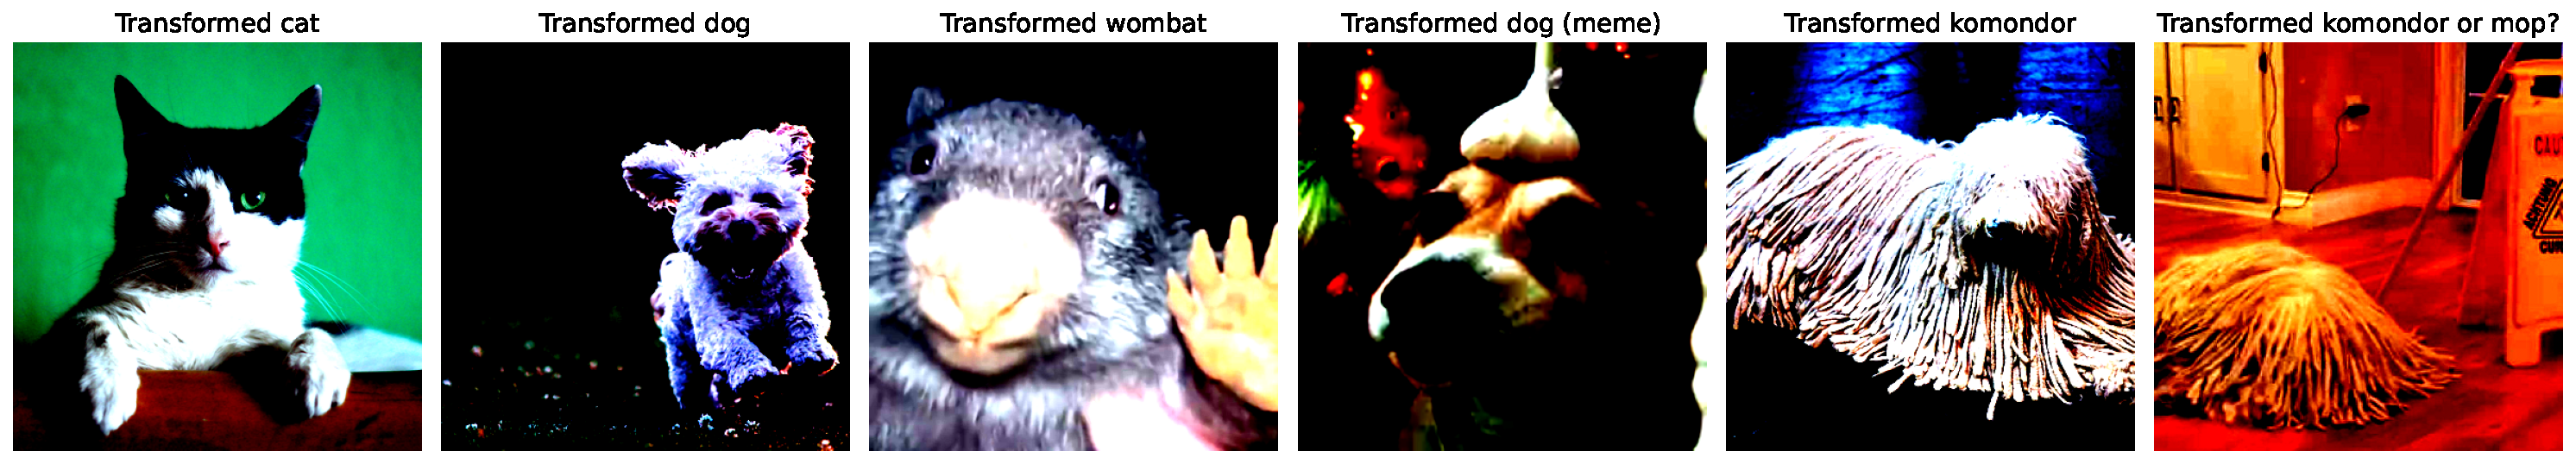
\includegraphics[width=\textwidth]{transformed_images_vit_bis}
        \caption{}
        \label{subfig:transformed_images_vit_bis}
    \end{subfigure}
    \begin{subfigure}{0.95\textwidth}
        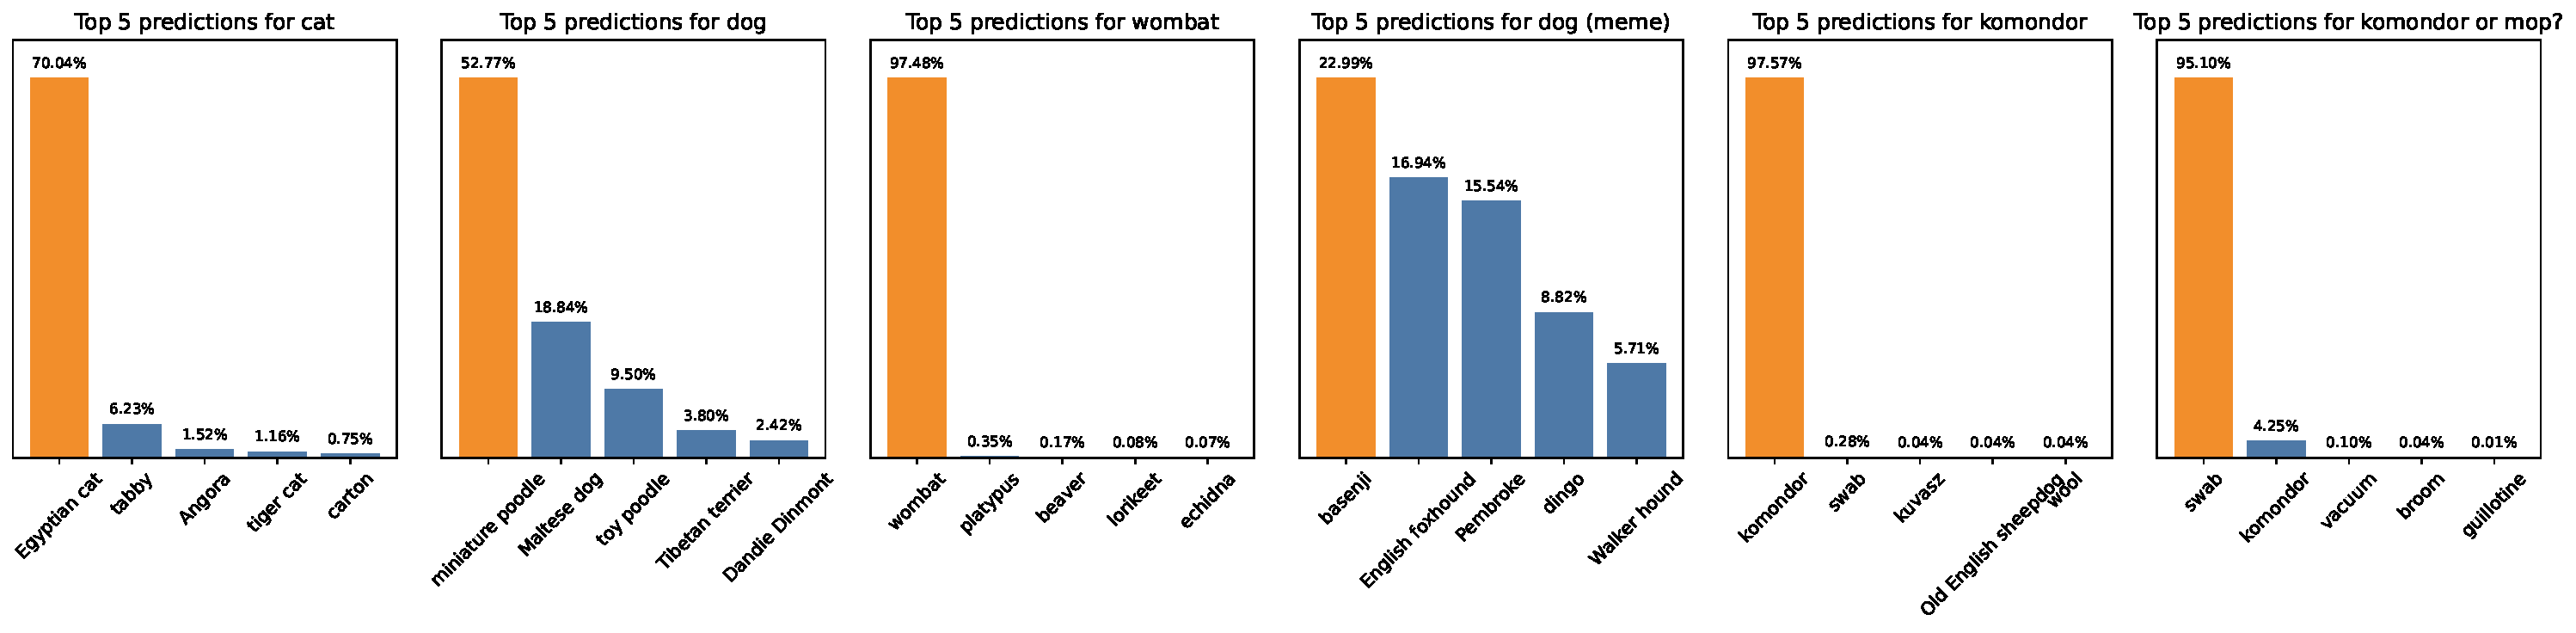
\includegraphics[width=\textwidth]{prediction_plots_vit_bis}
        \caption{}
        \label{subfig:prediction_plots_vit_bis}
    \end{subfigure}
    \caption{Performance evaluation of VisionTransformer pre-trained on ImageNet (IMAGENET1K\_SWAG\_E2E\_V1 weights): (a) Original images, (b) Transformed images normalized and resized to $224 \times 224$, and (c) Top 5 predicted classes}
    \label{fig:vit_refined}
\end{figure}